\begin{frame}{Highlevel Front-End Development}

    In general, Front-End developement  cover merely these two things.

    \begin{enumerate}
        \item  $ F_1(S) = U $ : Translate raw data to fancy UI.
        \item  $ F_2(S_{old},A)=S_{new} $ : Map user action to state transform.
    \end{enumerate}

    \begin{itemize}
        \pause
        \item \textbf{S}: Page State 
        \pause
        \item \textbf{U}: User Interface (e.g. Html and CSS)
        \pause
        \item \textbf{A}: User Actions. (e.g. click a button)
        \pause
        \item \textbf{$F_x$}: The code you write.
    \end{itemize}

    \pause


    

    
\end{frame}

\begin{frame}{Design Pattern for UI Development}

    The most difficult part of fe-dev is how to \textbf{manage} the \textbf{state}

    \pause
    There are lots of tries to solve  this problem

    \begin{itemize}
        \pause[2]
        \item MVC Framework: Django , Rails, JSP...
        \pause[3]
        \item MVVM Framework: Vue, WPF
    \end{itemize}

    \begin{columns}
        \pause[2]
        \begin{column}{.3\textwidth}
            \begin{figure}
                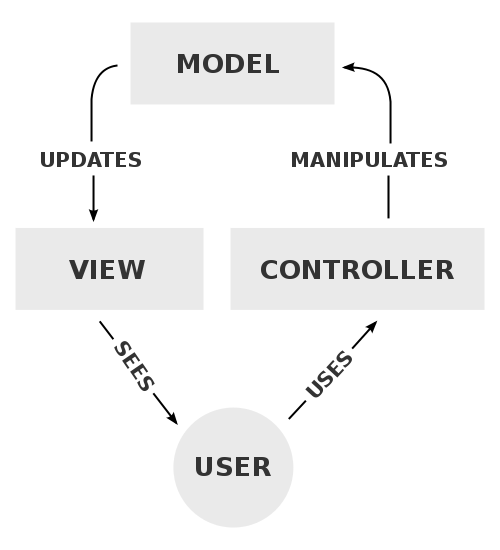
\includegraphics[width=\textwidth]{assets/MVC.png}
                \caption{MVC}
            \end{figure}
        \end{column}
    \pause[3]
        \begin{column}{.7\textwidth}
            \begin{figure}
                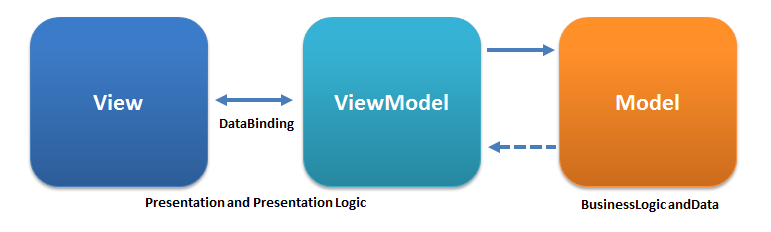
\includegraphics[width=\textwidth]{assets/MVVM.png}
                \caption{MVVM Diagram }
            \end{figure}
        \end{column}
    \end{columns}
\end{frame}

\begin{frame}{Let's Play React}
    React is neither MVC nor MVVM.
 
    \pause 
    React is a tool help you to develop $F_1$ and $F_2$
    \begin{itemize}
        \item JSX/TSX:  easily render state to HTML/CSS. $F_1$
        \item Hooks: manage the state gracefully 
        \item React Bubble Event: Shimming layer over raw DOM event.
    \end{itemize}


\end{frame}